\chapter{Vyhodnocení tří detektorů stop v pevné fázi}
\begin{wrapfigure}{r}{0.42\textwidth}
%\begin{figure}[h]
  \centering
  %\vspace{-20pt}
  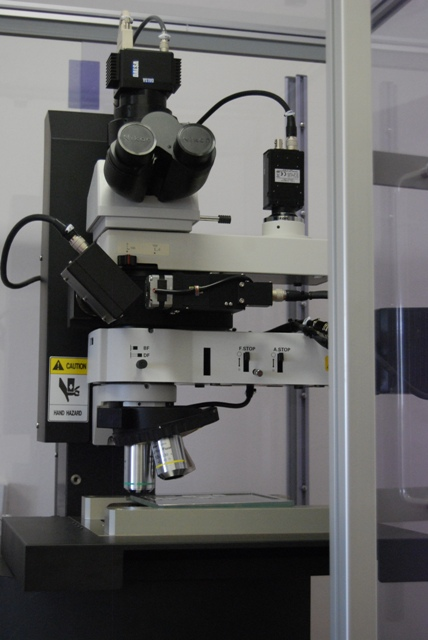
\includegraphics[width=0.4\textwidth]{praktickaCast_mikroskop}
  %\vspace{-20pt}
  \caption{Vysoko rychlostní optický mikroskop HSP-1000. \cite{dosis_HSP1000}}
  \label{fig:praktickaCast_mikroskop}
  \vspace{-10pt}
%\end{figure}
\end{wrapfigure}
V praktické části bakalářské práce byly vyhodnoceny tři detektory stop osmé sady experimentu DOSIS3D, které byly součástí prvního, druhého a třetího PDP. Jedná se o detektory z materiálu Tastrak, které byly leptány 6 hodin, tj. zobrazené stopy jsou původem od částic s krátkým dosahem a vyšším LET. Povrch detektorů byl již nasnímám, vyhodnocení detektorů tedy započalo analýzou stop v programu HspFit. Tento program sám vyhodnotí a zaznamená při dobrém nastavení určitých parametrů většinu stop, zbytek se musí označit ručně, což je zdlouhavá práce. Stopy se zaznamenávají tak, že se jejich okraj fituje elipsou, přičemž parametry fitu představují osy elipsy (hlavní $a$ a vedlejší $b$). V případě špatného automatického fitu lze proklad opravit ručně. Na obr.~\ref{fig:praktickaCast_hspfit} vidíme okno programu HspFit, zeleně jsou označeny stopy zaznamenané počítačem, červeně stopy zaznamenané uživatelem a fialově opravené fity. Dále lze
pozorovat, že některé stopy ještě na zaznamenání čekají. 

Na obr.~\ref{fig:praktickaCast_mikroskop} je mikroskopický systém HSP-1000 (neúplný, chybí počítač, který systém řídí) pomocí něhož byl povrch detektorů nasnímkován v dostatečném přiblížení.
\begin{figure}[ht]
  \centering
  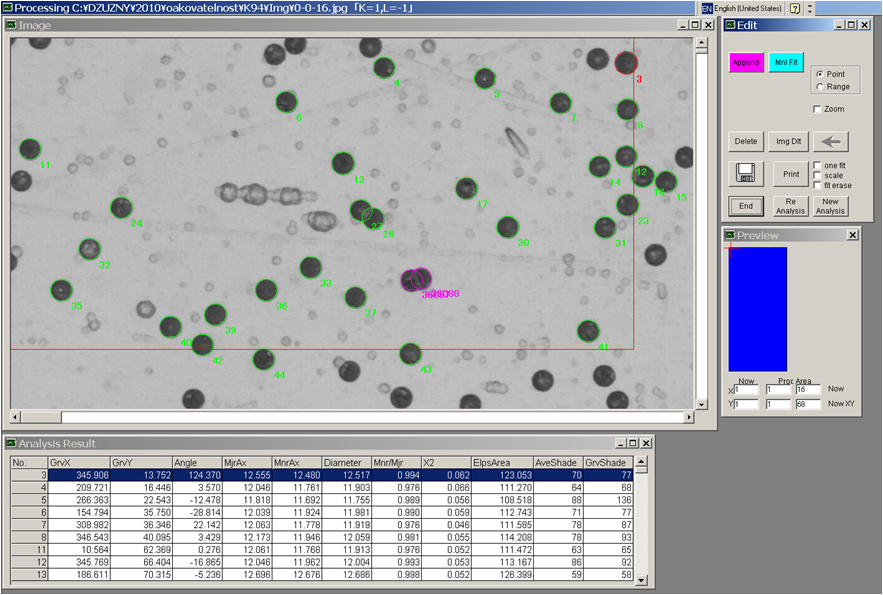
\includegraphics[width=0.85\textwidth]{praktickaCast_hspfit}
  \caption{Okno programu HspFit; zeleně jsou označeny fity vygenerované počítačem, fialově opravené fity uživatelem a červeně fity vytvořené uživatelem. \cite{dosis_HSP1000}}
  \label{fig:praktickaCast_hspfit}
\end{figure}

V obr. \ref{fig:praktickaCast_stopy} jsou uvedeny jednotlivé snímky z povrchu náhodně vybraného detektoru. V (a) je snímek, který obsahuje v čisté stopy; v (b) ukazuje červená šipka poškození materiálu, které by mohl neznalý uživatel vyhodnotit jako vícero stop; v (c) taktéž ukazuje červená šipka poškození materiálu, ale jiného charakteru. Obr.~\ref{fig:praktickaCast_stopyPoskozeni} pak ukazuje snímky, na nichž je naskenována plocha, která byla fyzicky znehodnocena člověkem (označení detektoru vyrytím X). 
\begin{figure}[h]
  \centering
  \begin{subfigure}{0.7\textwidth}
	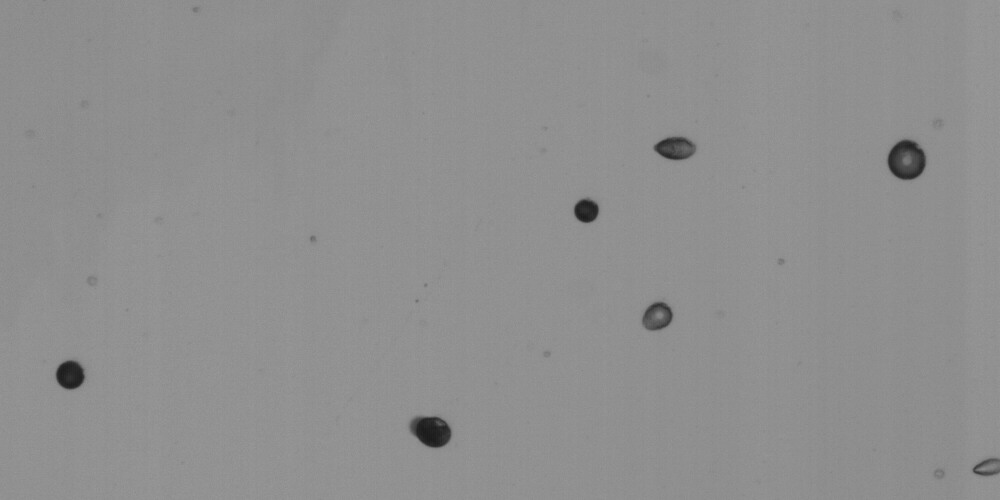
\includegraphics[width=\textwidth]{praktickaCast_stopyOK.jpg}
	\caption{}
  \end{subfigure}
  \begin{subfigure}{0.7\textwidth}
	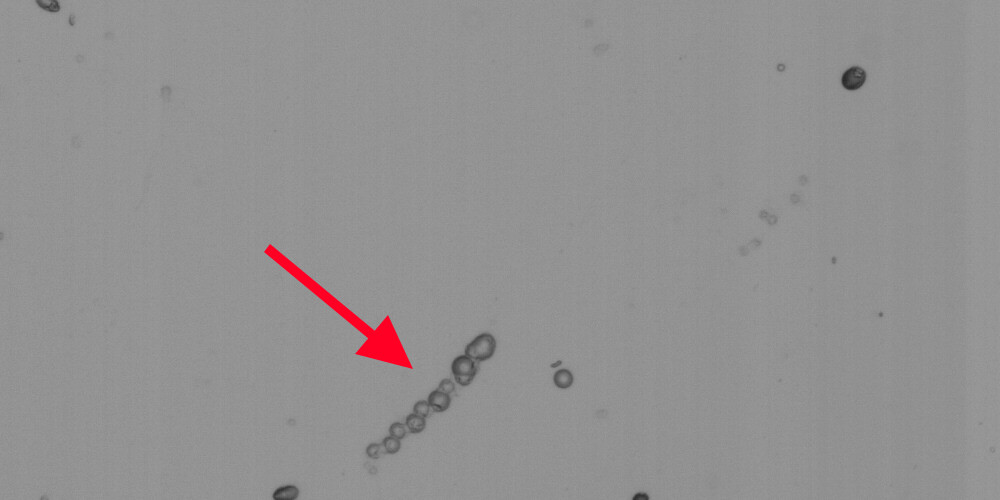
\includegraphics[width=\textwidth]{praktickaCast_stopyNeniStopa1.jpg}
	\caption{}
  \end{subfigure}
  \begin{subfigure}{0.7\textwidth}
	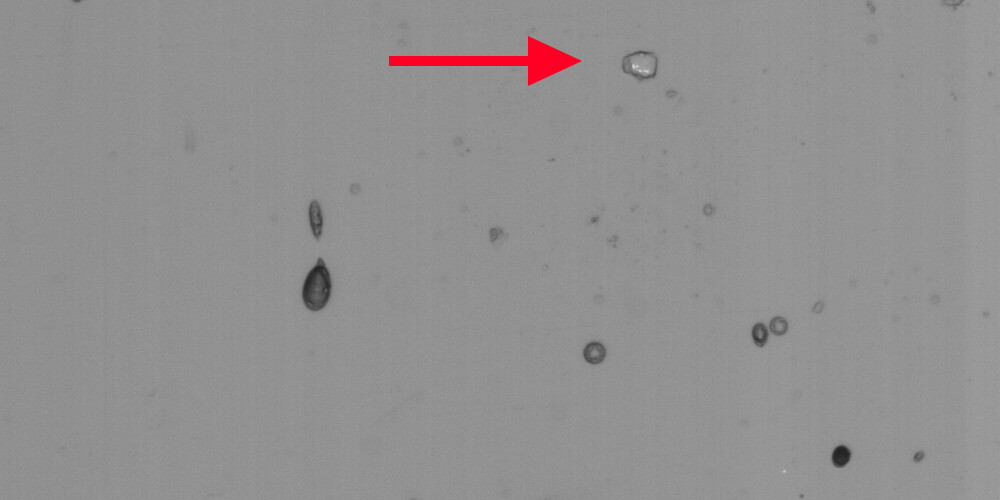
\includegraphics[width=\textwidth]{praktickaCast_stopyNeniStopa2.jpg}
	\caption{}
  \end{subfigure}
  \caption{Příklad naskenovaných snímků jednoho detektoru. V (a) jsou vidět normální stopy, v (b) a (c) naopak červené šipky ukazují na poškození materiálu, která nevznikla působením ionizujícího záření.}
  \label{fig:praktickaCast_stopy}
\end{figure}
\begin{figure}[h]
  \centering
  \begin{subfigure}{0.7\textwidth}
	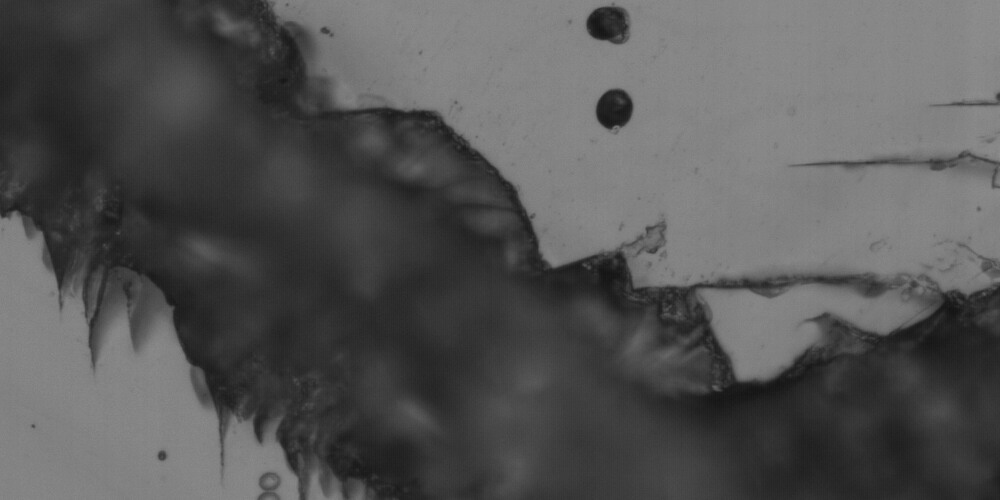
\includegraphics[width=\textwidth]{praktickaCast_stopyPoskozeni1.jpg}
	\caption{}
  \end{subfigure}
  \begin{subfigure}{0.7\textwidth}
	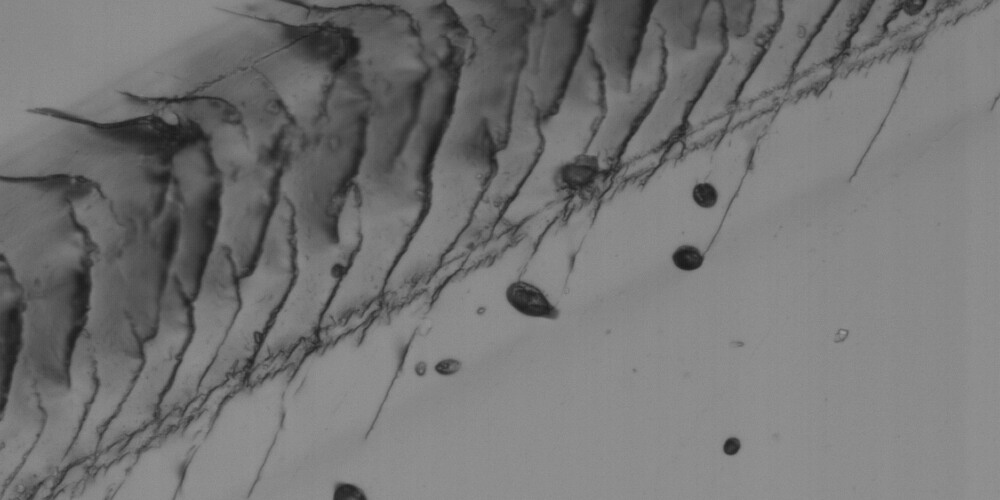
\includegraphics[width=\textwidth]{praktickaCast_stopyPoskozeni2.jpg}
	\caption{}
  \end{subfigure}
  \caption{Naskenované snímky zobrazující poškozené části plochy detektoru vyrytím značky X.}
  \label{fig:praktickaCast_stopyPoskozeni}
\end{figure}

Osy všech elips byly spolu s dalšími parametry fitů (např. sklon elipsy) uloženy v souboru s příponou .nap. Tyto data byla zpracována skriptem napsaném v programovacím jazyce Python, jehož výstupem jsou dva soubory a jeden graf. První soubor obsahuje údaje o poloze stopy, os fitované elipsy, poměru leptacích rychlostí $V$, korekčním součiniteli $k_{\theta}$, lineárním přenosu energie $\LET$, dávce $D_i$ a dávkovém ekvivalentu $H_i$ každé stopy. Druhý soubor obsahuje celkovou dávku a dávkový ekvivalent, které se absorbovaly v detektoru; dále obsahuje data potřebná k vytvoření diferenciálního $\LET$ spektra; z těchto dat je vytvořen výstupní graf. Skript vypočítává pro každou částici $V$ z hodnot $a,b$ (vztah \eqref{eq:pomerLepRychlosti}, tloušťka odleptané vrstvy je $7,5$
$\mu$m) a následně $\LET$ dané částice z $V$ pomocí kalibrační křivky pro TASTRAK leptaný 6 hodin. Tato i druhá kalibrační křivka pro TASTRAK leptaný 15 hodin jsou tvaru
\begin{align}
  \LET(V) &= -99,8424+125,00172  V-15,28166  V^2+2,04636  V^3\quad\text{(6 hod)},\label{eq:kalibracniKrivkaSestHod}\\
  \LET(V) &= -96,35071+114,90343  V-7,77194  V^2+1,27248  V^3\quad\text{(15 hod)},\label{eq:kalibracniKrivkaPatnactHod}
\end{align}
kde $\LET$ vychází v keV/$\mu$m; závislosti byly přebrány z \cite{ssntd}. Z $\LET$ částice je dále vypočítána dávka předaná danou částicí $D_i$ ze zjednodušeného vztahu \eqref{eq:Davka} 
\begin{equation}
  D_i=\text{konst}\cdot\LET\cdot k_{\theta}\cdot\frac{2}{ProcArea}\,, 
  \label{eq:praktickaCast_davkaJednaCastice}
\end{equation}
kde $\text{konst}=1,602\cdot 10^{-6}$, $ProcArea$ <++?++>. Dávkový ekvivalent od dané částice $H_i$ je určen ze vztahu 
\begin{equation}
  H_i=D_i\cdot Q\,.
  \label{eq:praktickaCast_ekvDavkaJednaCastice}
\end{equation}
$Q$ je jakostní faktor určený podle ICRP 60 (tab. \ref{tab:detektory_Q}). Celková dávka $D$ a dávkový ekvivalent $H$ jsou $D_i$ a $H_i$ všech částic. 

V tab. \ref{tab:praktickaCast_davkyVysledky} jsou celkové dávky a dávkové ekvivalenty určené třemi vyhodnocenými detektory Na obr. \ref{fig:praktickaCast_LETspektra} jsou $\LET$ spektra získaná z vyhodnocených detektorů.
%osmá sada
\begin{table}[h]
  \centering
  \caption{Celkové dávky $D$ a dávkové ekvivalenty $H$ určené vyhodnocovanými detektory.}
  \label{tab:praktickaCast_davkyVysledky}
  \begin{tabular}{lll}
	\toprule
	PDP&$D$ [mGy]&$H$ [mSv]\\
	\midrule
	%1&5,31501450067&88,2754298605\\
	%2&5,068573344&92,5692674847\\
	%3&4,31129592097&75,4191405129\\
	1&5,3150&88,2754\\
	2&5,0686&92,5693\\
	3&4,3113&75,4191\\
	\bottomrule
  \end{tabular}
\end{table}
\begin{figure}[h]
  \centering
  \begin{subfigure}{0.49\textwidth}
	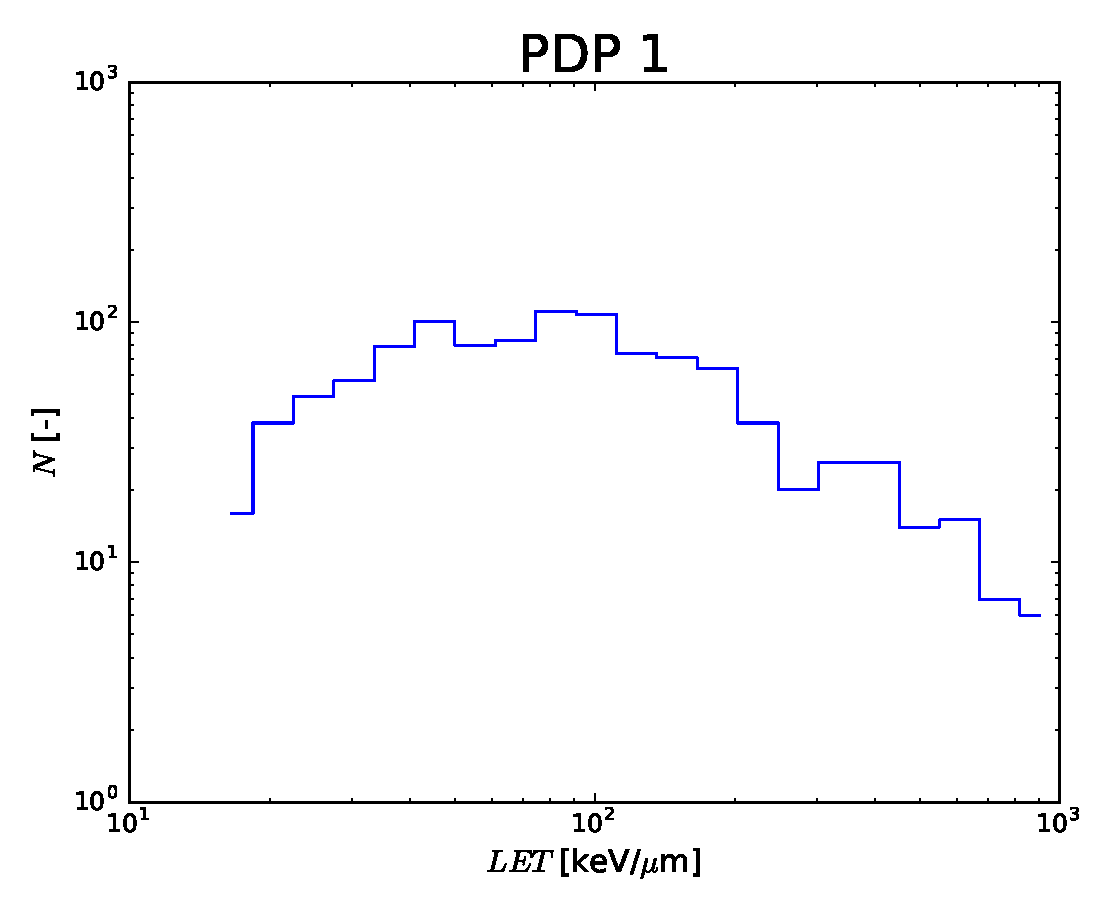
\includegraphics[width=\textwidth]{praktickaCast_spektrum1.eps}
	\caption{}
  \end{subfigure}
  \begin{subfigure}{0.49\textwidth}
	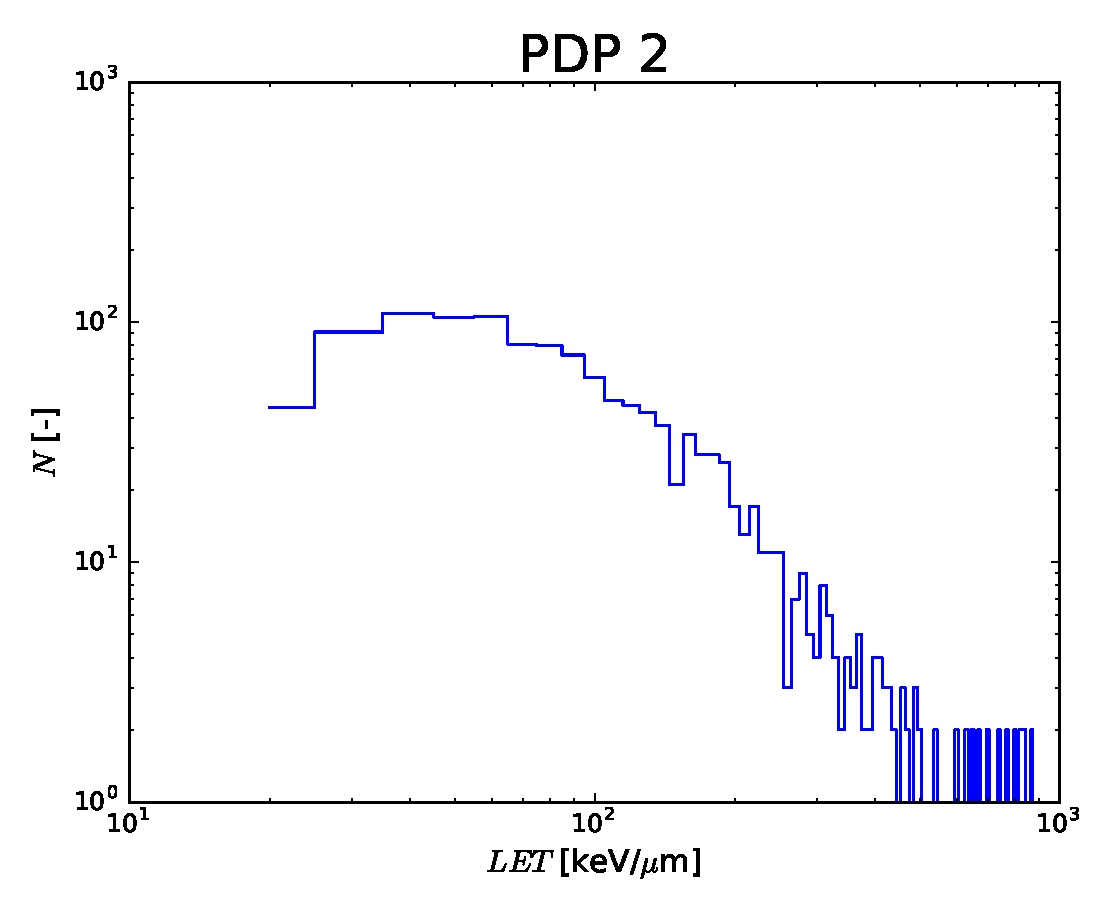
\includegraphics[width=\textwidth]{praktickaCast_spektrum2.eps}
	\caption{}
  \end{subfigure}
  \begin{subfigure}{0.49\textwidth}
	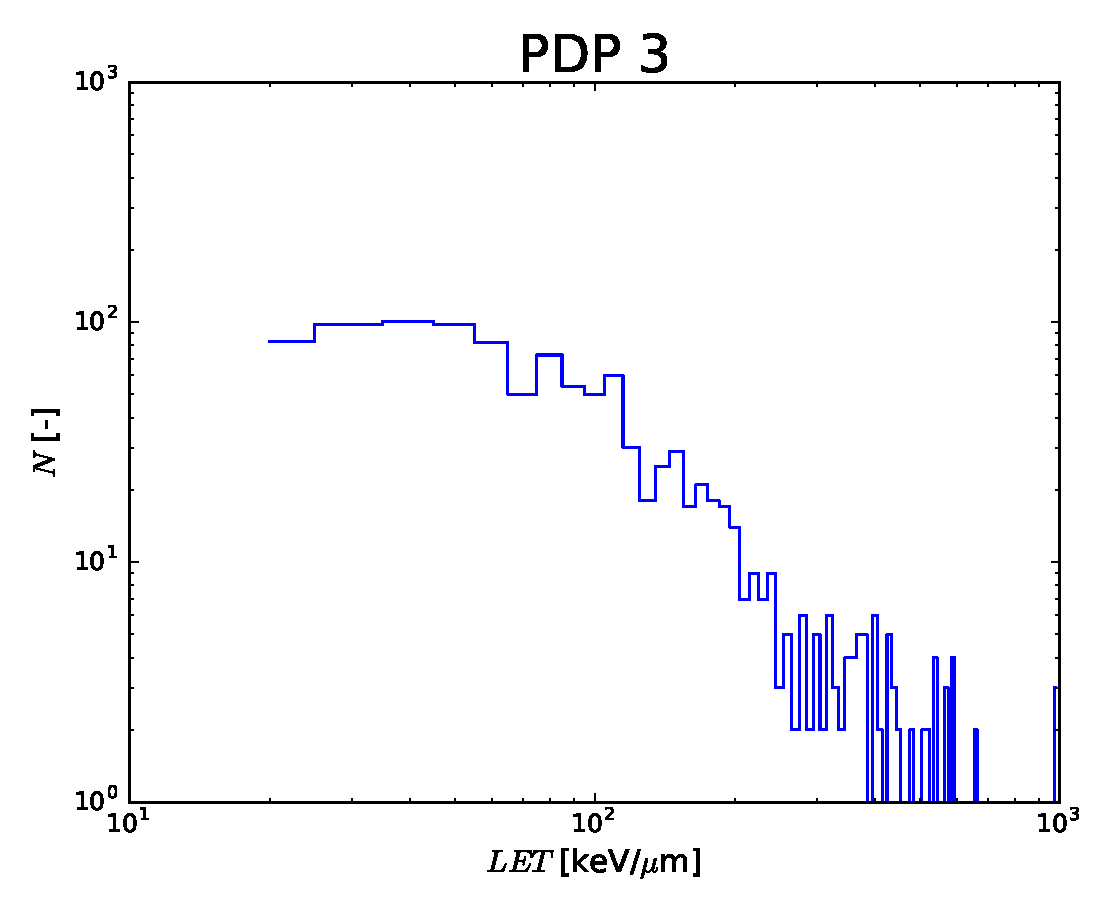
\includegraphics[width=\textwidth]{praktickaCast_spektrum3.eps}
	\caption{}
  \end{subfigure}
  \caption{Diferenciální $\LET$ spektra vyhodnocených detektorů. Na svislé ose je počet impulzů spadnuvších do příslušného kanálu.}
  \label{fig:praktickaCast_LETspektra}
\end{figure}

